\documentclass[14pt,usenames,dvipsnames,svgnames]{beamer}
\usepackage[english]{babel}
\usepackage[misc]{ifsym}
\usepackage{mathspec,mathabx,multicol,listings,comment,fontawesome,pgfornament,comment}
\usepackage{TeXnicalities}
\usetikzlibrary{shapes}

\setsansfont{Yanone Kaffeesatz}[
    UprightFont     = *-Regular ,
    BoldFont        = *-Bold ,
    BoldItalicFont  = *-Bold ,
    BoldSlantedFont = *-Bold ,
    ItalicFont      = *-Light ,
    SlantedFont     = *-Light ,
    SmallCapsFont   = *-Thin
]

\graphicspath{{Figures/}}
\usepackage{listings}
\def\transpPerc{100}
%listings set
\lstdefinestyle{MyCpp}{
% backgroundcolor=\color{white},    % choose the background color; you must add \usepackage{color} or \usepackage{xcolor}
breakatwhitespace=false,            % sets if automatic breaks should only happen at whitespace
breaklines=true,                    % sets automatic line breaking
captionpos=b,                       % sets the caption-position to bottom
deletekeywords={...},               % if you want to delete keywords from the given language
escapeinside={@|}{|@},                % if you want to add LaTeX within your code
extendedchars=true,                 % lets you use non-ASCII characters; for 8-bits encodings only,
                                    % does not work with UTF-8
frame=none  ,                       % adds a frame around the code
numbers=none,                       % where to put the line-numbers; possible values are (none, left, right)
numbersep=5pt,                      % how far the line-numbers are from the code
numberstyle=\tiny\color{black},     % the style that is used for the line-numbers
rulecolor=\color{black},            % if not set, the frame-color may be changed on line-breaks within not-black text
                                    % (e.g. comments (green here))
showspaces=false,                   % show spaces everywhere adding particular underscores; it overrides 'showstringspaces'
showstringspaces=false,             % underline spaces within strings only
showtabs=false,                     % show tabs within strings adding particular underscores
stepnumber=2,                       % the step between two line-numbers. If it's 1, each line will be numbered
stringstyle=\color{OliveGreen},     % string literal style
tabsize=2,                          % sets default tabsize to 2 spaces
title=\lstname,                     % show the filename of files included with \lstinputlisting; also try caption instead of title
%
%Base style for this presentation 
keepspaces=true,                    % keeps spaces in text, useful for keeping indentation of code
                                    % (possibly needs columns=flexible)
keywordstyle=\color{Cyan},          % keyword style
language=C++,
basicstyle=\ttfamily\scriptsize\color{black},
keywordstyle=\color{OliveGreen},
stringstyle=\color{Magenta},
commentstyle=\color{red},
moredelim=[is][\color{ForestGreen}]{|+}{+|},
literate=% literate={<replace>}{<replacement text>}{<width>}
  {\#define}{{{\color{CarnationPink}\#define}}}{6}
  {\#include}{{{\color{CarnationPink}\#include}}}{7},
morekeywords={real, vector, Minesweeper, myVecVec, Cell, SetOfCells, regex, T, string, CD,
              invalid_argument, Jukebox, Coffee, Version, Point2D, Point3D, Person, pair},
emph=[1]{calculateAverage, size, exit, begin, end, find, makeReportForUser, isElementInVector,
         main, WelcomeUserToTheGame, playGame, PrintGameResult, isPrime, sqrt, push_back, FC,
         getFlaggedCells, isFlagged, at, isEligibleForFullBenefits, gsl_fcmp, getDefaultForHelper,
         trim_right, addCD, MakeCoffee, WarmUpMachineIfNeeded, GrindCoffee, SetPressureAndTemperature,
         BrewCoffee, getMajorVersionNumber, getMinorVersionNumber, getBuildNumber, Distance, factorial,
         Q_rsqrt, Q_fastInverseSqrt, calculateApproximateInverseSqrt, refineResult, get, fetch, retrieve, obtain},
emphstyle=[1]{\color{NavyBlue}}, %Functions
emph=[2]{cout, data, sum, sum1, sum2, data, dataSet, dataSet1, dataSet2, first, last, argc, argv, minesweeper,
         number, i, c, f, b, list, gameBoard, flaggedCells, cell, realDaysPerIdealWeek, totalRealWeeksNeeded,
         realDaysPerTask, taskDaysEstimate, realWeeksPerTask, j, e, employee, timePattern, iterationNumber,
         functionValue, epsilon, it, value, keyToDecipher, longTitle, longAuthor, durationInMinutes, cd,
         typeOfCoffee, x, y, z, x2, approximateResult, floatAsInteger, initialNumber, refinedResult,
         threehalfs, result, timestamp, ymdhms},
emphstyle=[2]{\color{Orange}}, %Variables
emph=[3]{if, else, while, do, for, case, switch},
emphstyle=[3]{\color{violet}}, %Loops, if, etc.
emph=[4]{const, auto, break, continue, default, static, return, struct, NULL, sizeof, typedef,
         template, typename, true, false, throw, public, class},
emphstyle=[4]{\color{ProcessBlue}}, %Logical keywords
emph=[5]{std, boost},
emphstyle=[5]{\color{Maroon}}, %Namespaces
emph=[6]{STATUS_VALUE, FLAGGED, WORKING_DAYS_PER_WEEK, NUMBER_OF_TASKS, HOURLY_FLAG,
         CG_CHECK_RESIDUUM_EVERY, BOOST_AUTO_TEST_CASE, BOOST_TEST_MODULE, BOOST_REQUIRE_EQUAL},
emphstyle=[6]{\color{Gray}}, %Macros
emph=[7]{age, flags, title, author, tracks, duration, cdList},
emphstyle=[7]{\color{Peach!50!Purple}}, %Members
emph=[8]{Factorial, SpecialCases, NormalCases},
emphstyle=[8]{\color{Blue}}, %Boost cases and suite
}


\def\CPP{\lstinline[style=MyCpp, basicstyle=\ttfamily\color{black}]}

\makeatletter
\newenvironment{CenteredBox}{% 
\begin{Sbox}}{% Save the content in a box
\end{Sbox}\centerline{\parbox{\wd\@Sbox}{\TheSbox}}}% And output it centered
\makeatother


\usetikzlibrary{fadings}

\pgfkeys{%
/piechartthreed/.cd,
scale/.code                =  {\def\piechartthreedscale{#1}},
mix color/.code            =  {\def\piechartthreedmixcolor{#1}},
background color/.code     =  {\def\piechartthreedbackcolor{#1}},
name/.code                 =  {\def\piechartthreedname{#1}}}

\newcommand\piechartthreed[2][]{% 
   \pgfkeys{/piechartthreed/.cd,
     scale            = 1,
     mix color        = white,
     background color = white,
     name             = pc} 
  \pgfqkeys{/piechartthreed}{#1}
  \begin{scope}[scale=\piechartthreedscale] 
  \begin{scope}[xscale=5,yscale=3] 
     \path[preaction={fill=black,opacity=.8,
         path fading=circle with fuzzy edge 20 percent,
         transform canvas={yshift=-15mm*\piechartthreedscale}}] (0,0) circle (1cm);
    \fill[gray](0,0) circle (0.5cm);  
     \path[preaction={fill=\piechartthreedbackcolor,opacity=.8,
          path fading=circle with fuzzy edge 20 percent,
          transform canvas={yshift=-10mm*\piechartthreedscale}}] (0,0) circle (0.5cm);
     \pgfmathsetmacro\totan{0} 
     \global\let\totan\totan 
     \pgfmathsetmacro\bottoman{180} \global\let\bottoman\bottoman 
     \pgfmathsetmacro\toptoman{0}   \global\let\toptoman\toptoman 
     \begin{scope}[draw=black,thin]
     \foreach \an/\col [count=\xi] in {#2}{%
     \def\space{ } 
        \coordinate (\piechartthreedname\space\xi) at (\totan+\an/2:0.75cm); 
        \ifdim 180pt>\totan pt 
         \ifdim 0pt=\toptoman pt
            \shadedraw[left color=\col!50!\piechartthreedmixcolor,
                       right color=\col!25!\piechartthreedmixcolor,
                       draw=black,very thin] (0:.5cm) -- ++(0,-3mm) arc (0:\totan+\an:.5cm) 
                                                       -- ++(0,3mm)  arc (\totan+\an:0:.5cm);
            \pgfmathsetmacro\toptoman{180} 
            \global\let\toptoman\toptoman         
            \else
            \shadedraw[left color=\col!50!\piechartthreedmixcolor,
                       right color=\col!25!\piechartthreedmixcolor,
                       draw=black,very thin](\totan:.5cm)-- ++(0,-3mm) arc(\totan:\totan+\an:.5cm)
                                                        -- ++(0,3mm)  arc(\totan+\an:\totan:.5cm); 
          \fi
        \fi   
        \fill[\col,draw=black] (\totan:0.5cm)--(\totan:1cm)  arc(\totan:\totan+\an:1cm)
                                     --(\totan+\an:0.5cm) arc(\totan+\an:\totan :0.5cm);     
       \pgfmathsetmacro\finan{\totan+\an}
       \ifdim 180pt<\finan pt 
         \ifdim 180pt=\bottoman pt
            \shadedraw[left color=\col!50!\piechartthreedmixcolor,
                       right color=\col!25!\piechartthreedmixcolor,
                       draw=black,very thin] (180:1cm) -- ++(0,-3mm) arc (180:\totan+\an:1cm) 
                                                       -- ++(0,3mm)  arc (\totan+\an:180:1cm);
            \pgfmathsetmacro\bottoman{0}
            \global\let\bottoman\bottoman
            \else
            \shadedraw[left color=\col!50!\piechartthreedmixcolor,
                       right color=\col!25!\piechartthreedmixcolor,
                       draw=black,very thin](\totan:1cm)-- ++(0,-3mm) arc(\totan:\totan+\an:1cm)
                                                        -- ++(0,3mm)  arc(\totan+\an:\totan:1cm); 
          \fi
        \fi
        \pgfmathsetmacro\totan{\totan+\an}  \global\let\totan\totan 
       } 
    \end{scope}
    \draw[thin,black](0,0) circle (0.5cm);
   \end{scope}  
\end{scope}
}



%Tikz
\tikzset{
    %Hexagons
    hexagon/.style n args={3}{double arrow, double arrow head extend=0cm, inner sep=3pt, draw=#1, fill=#2, text=#3, thick},
    hexagon/.default={black}{gray!20}{black},
    hexagonOne/.style={hexagon={#1}{#1!30}{#1}},
    hexagonTwo/.style 2 args={hexagon={#1}{#1!#2}{#1}},
    hexagonThree/.style n args={3}{hexagon={#1}{#1!#2}{#3}},
    hexagonShade/.style n args={3}{double arrow, double arrow head extend=0cm, inner sep=3pt, thick, draw=#1, left color=#2, right color=#3},
    %General text element
    Shape/.style n args={3}{draw=#1, fill=#2, text=#3},
    genShape/.style 2 args={#1, inner sep=3pt, draw=#2, fill=#2!20, text=#2, thick},
    halo/.style={preaction={draw, #1, line width=7, -}},
}

%My commands
\newcommand<>{\tc}[2]{\textcolor#3{#1}{#2}}
\newcommand{\myCopyright}{\raisebox{-7pt}{\large\copyright}}
\makeatletter
    \newlength{\textsize}
    \setlength{\textsize}{\f@size pt}
    \newcommand{\emoji}[1]{\;\raisebox{-0.15\textsize}{\includegraphics[height=\f@size pt]{#1}}}
\makeatother


\makeatletter
\patchcmd{\beamer@sectionintoc}
  {\vfill}
  {\vskip\itemsep}
  {}
  {}
\makeatother

\mode<presentation>
{
    \usetheme{Z02}
    \defbeamertemplate{footline}{Empty}{}
    \setbeamersize{text margin left=5mm,text margin right=5mm}
}

%===============================================================%
\title{Clean testing}
\subtitle{Good practices in general coding}
\author{Alessandro Sciarra}
\institute{Z02~--~Software Development Center}
\date{XX July 2023}
\titlegraphic{
\includegraphics[width=25mm]{LogoCRC}}
\titlepagelogo{
\includegraphics[width=25mm]{LogoGoethe}}
%===============================================================%

\AtBeginSection[] % <- Empty optional argument, do nothing for \section*
{
    \begin{frame}[plain, noframenumbering]{}
         \sectionpage
    \end{frame}
}
\begin{document}
\begin{comment}
%===================================================================================================%
\begin{frame}[plain,noframenumbering]
    \titlepage
\end{frame}
%~~~~~~~~~~~~~~~~~~~~~~~~~~~~~~~~~~~~~~~~~~~~%
\begin{frame}[plain,noframenumbering]{Prelude}
    \begin{equation*}
        \text{The slides will be available on the web}\,
        \left\{
        \begin{aligned}
            &\text{\URL[PB]{https://th.physik.uni-frankfurt.de/~strongmatter/\#Seminars}{CRC-TR211}} \\
            &\text{\URL[PP]{https://github.com/AxelKrypton}{\faGithub\,AxelKrypton}} \\
        \end{aligned}
        \right.
    \end{equation*}
    \vspace{-3mm}
    \begin{varblock}{block example}[0.8\textwidth]{Leave me a feedback}
        Was the talk clear, useful, inspiring?\\
        Any general comment? $\quad$
        \tc{PP}{\href{mailto:sciarra@th.physik.uni-frankfurt.de}{{\small\Letter}$\;$Alessandro}}
    \end{varblock}
    \vspace{1mm}
    \PrepareURLsymbol[PT]
    \begin{varblock}{block alerted}[0.9\textwidth]{Disclaimer}
        Slides are quite full of text for later reading. \\
        Most example to fit on a slide are oversimplified.\\
        Tests shown before BDD/TDD sections are probably bad.\\[1mm]
        $\Rightarrow\,$ \textbf{Let's discuss!}
    \end{varblock}
\end{frame}
%~~~~~~~~~~~~~~~~~~~~~~~~~~~~~~~~~~~~~~~~~~~~%
\begin{frame}[plain,noframenumbering]{Outline}
    \vspace{-3mm}
    \hspace*{1cm}
    \begin{minipage}[0.65\textheight]{\textwidth}
        \tableofcontents
    \end{minipage}
\end{frame}
%===================================================================================================%


%===================================================================================================%
\section{A short recap about clean code}
%~~~~~~~~~~~~~~~~~~~~~~~~~~~~~~~~~~~~~~~~~~~~%
\begin{frame}{What we explored in the clean code talk}
    \begin{itemize}
        \item Take advantage of your IDE
        \item Use meaningful names
        \item Limit comments and care about formatting
        \item Function and classes should have a single responsibility (SRP)
        \item Integration Operation Separation Principle (IOSP)
        \item Don't repeat yourself (DRY)
        \item Keep it simple, stupid (KISS)
        \item Beware of optimisation
        \item The boyscout rule
        \item Keep improving
    \end{itemize}
    \begin{tikzpicture}[remember picture, overlay]
        \node[anchor=south east, inner sep=5mm] (fig) at (current page.south east)
            {
\includegraphics[width=0.5\textwidth]{Bifurcation}};
        \node[text=BGLIGHT, font=\Large\bfseries] at ($(fig.center)!0.3!(fig.south)+(0.05,0)$)
            {
                \begin{tabular}{c}
                    Develop\\[-2mm]
                    your code sense\\
                \end{tabular}
            };
    \end{tikzpicture}
\end{frame}
%===================================================================================================%


%===================================================================================================%
\section{Why (automated) testing?}
%~~~~~~~~~~~~~~~~~~~~~~~~~~~~~~~~~~~~~~~~~~~~%
\begin{frame}{Lots of software should rather work...}{In our society you cannot spend 60 seconds without interacting with a software system}
    \vspace{-2mm}
    \begin{enumerate}
        \item \parbox[t]{0.5\textwidth}{In modern car there is software that controls the steering wheel\ldots}
              \qquad\raisebox{-.5\height}{
\includegraphics[width=22mm]{Lane_assistant_symbol}}
        \item Think of medical devices, aeroplanes, lifts, etc.
        \item Aren't you upset when an app on your phone stalls or crashes?!
    \end{enumerate}
    \vspace{2mm}
    \begin{varblock}{example}[\textwidth]{An remarkable story about manual testing}<uncover@2->
        I have been using an own manually tested ``agenda-script'' to track my working time \alert{\textbf{for months}} and then one day it suddenly crashed.\\
        Where was the problem?
        \uncover<3>{\PB{I assumed \textbf{every} day has 24 hours\ldots\emoji{Innocent}}}
    \end{varblock}
\end{frame}
%~~~~~~~~~~~~~~~~~~~~~~~~~~~~~~~~~~~~~~~~~~~~%
\newcommand{\FermatExample}[4][3]{$#2^#1+#3^#1\neq#4^#1$}
\begin{frame}{The unfortunate tendency in many cases}
    \vspace{-3mm}
    \begin{itemize}
        \item \alert{It gives reasonable results, it works!} \emoji{Scream}
        \item Manual (and possibly not systematic) testing is unfortunately still common practice in our community!
        \item Even if done in a systematic way, you will never run your tests enough!
    \end{itemize}
    \begin{overlayarea}{\textwidth}{0.4\textheight}
        \begin{onlyenv}<1>
            \begin{varblock}{quote}[0.7\textwidth]{Theorem:}
                Prove that, with $n,x,y,z\in \mathbb{N}>0$ and $n>2$, the equation $x^n+y^n =z^n$ has no solutions.
            \end{varblock}
            \begin{varblock}{quote}[0.8\textwidth]{Would you accept this as proof or even argument?}
                \small
                \FermatExample{2}{3}{4}\; and\;\FermatExample[4]{1}{5}{6}\; and\;\FermatExample[5]{4}{2}{5}
            \end{varblock}
        \end{onlyenv}
        \begin{onlyenv}<2>
            \begin{varblock}{alert}[0.7\textwidth]{Now, software testing is not like mathematics...}
                \large ...but would you accept a physics fact \textbf{without rigorous evidence}?
            \end{varblock}
        \end{onlyenv}
    \end{overlayarea}
\end{frame}
%~~~~~~~~~~~~~~~~~~~~~~~~~~~~~~~~~~~~~~~~~~~~%
\begin{frame}{Consider one of your programs. Does it work?}
    \vspace{-5mm}
    \begin{varblock}{example}[0.8\textwidth]{How do you prove that a software works?}
        \uncover<2->{
            You don't.
            You try proving it doesn't work\ldots\ and fail!
        }
    \end{varblock}
    \begin{uncoverenv}<3>
        \begin{varblock}{}[\textwidth]{The scientific method}
            \begin{enumerate}
                \item Make an hypothesis $\PB{\;\mathcal{C}\;}\to\;$  «My code is correct»
                \item Tests attempt to show $\PB{\;!\mathcal{C}\;}$
                \item Confidence in $\;\PB{\mathcal{C}\;}$ tracks thoroughness of tests
            \end{enumerate}
        \end{varblock}
        \vspace{-2mm}
        \begin{varblock}{}[\textwidth]{}
            \large
            Testing code is science (cf. Popper's falsification principle)
        \end{varblock}
    \end{uncoverenv}
\end{frame}
%~~~~~~~~~~~~~~~~~~~~~~~~~~~~~~~~~~~~~~~~~~~~%
\begin{frame}{Uncle Bob's magic button}
    \begin{varblock}{quote}[1.02\textwidth]{Fearless competence}
        Are you afraid to touch the code?
        Are you afraid to improve the code?
        Do you have that little echo in your  ear saying -- Ah, if it ain't broken, don't fix it?
        I expect you to improve the code, all of the time, fearless competence.
        How do you get fearless competence?
    \end{varblock}
    \vspace{-3mm}
    \begin{center}
        \begin{tikzpicture}
            \node (button) {
\includegraphics[width=0.25\textwidth]{Magic_button}};
            \node[right = of button] (Y) {
\includegraphics[width=12mm]{Yes}};
            \node[left = of button] (N) {
\includegraphics[width=12mm]{X}};
            \path[to, thick] (button) edge[out=0, in=180] (Y);
            \path[to, thick] (button) edge[out=180, in=0] (N);
        \end{tikzpicture}
    \end{center}
    \vspace{-3mm}
    \begin{varblock}{quote}[0.95\textwidth]{}[Robert C. Martin]
        Tests! What if I had a button, a little button I could push on my keyboard and some lights would blink and science-fiction sounds would come out of my laptop for a few minutes and then a little green light would light up and that green light told me that the system worked.
        \alert{And I believed it.}
    \end{varblock}
\end{frame}
%~~~~~~~~~~~~~~~~~~~~~~~~~~~~~~~~~~~~~~~~~~~~%
\begin{frame}{The correct mental approach to testing}
    \begin{itemize}
        \setlength{\itemindent}{-2mm}
        \item Testing is part of the natural evolution of the code (not an overhead)
        \item Test code has to fulfil the same clean code rules as production code
        \item \alert{Tests are the key to be free to change (improve) the production code!}
        \item Keep balance between adding new code, writing tests and refactoring
    \end{itemize}
    \vspace{3mm}
    \begin{center}
        \resizebox{!}{0.32\textheight}{
            \begin{tikzpicture}
                \tikzstyle{Pie}=[font=\Large]
                \tikzstyle{PieNum}=[font=\Large\bfseries\ttfamily]
                \piechartthreed[scale=0.8,
                background color=white,
                mix color= white]{120/PS!50!LimeGreen,120/PP!50!white,120/PT}
                \foreach \i in {1,...,3} { \fill (pc \i) ellipse (0.1 and 0.05);}
                \draw[darkgray] (pc 1)  -- ++(7,0) coordinate (s1)
                node[Pie, anchor=south east] {Testing}
                node[PieNum, anchor=north east] {\tc{PS}{33\%}};
                \draw[darkgray] (pc 2)  -- ++(-1,1) -- ++(-5,0) coordinate (s2)
                node[Pie, anchor=south west] {Developing}
                node[PieNum, anchor=north west] {\tc{PP}{33\%}};
                \draw[darkgray] (pc 3)  -- (pc 3 -| s2)
                node[Pie, anchor=south west] {Refactoring}
                node[PieNum, anchor=north west] {\tc{PT}{33\%}};
            \end{tikzpicture}
        }
    \end{center}
    \FrameRemark{Slide taken from the \textsl{Clean Code} talk.}
    \begin{tikzpicture}[overlay, remember picture]
        \node[starburst, starburst points=27, starburst point height=16mm,
              minimum width=12cm, minimum height=5cm, Shape={red}{yellow!50}{red},
              line width=1.5pt, font=\Huge, rotate=10, visible on=<2>]
          at (current page.center) {Today much more!};
    \end{tikzpicture}
\end{frame}
%===================================================================================================%


%===================================================================================================%
\section{Different types of testing}
%~~~~~~~~~~~~~~~~~~~~~~~~~~~~~~~~~~~~~~~~~~~~%
\begin{frame}{Software testing}{Test code is just as important as production code}
    \vspace{-7mm}
    \begin{columns}[t]
        \begin{column}{0.45\textwidth}
            \begin{itemize}
                \item \PP{Testing levels}
                \begin{itemize}
                    \item \PS{Unit testing}
                    \item \PS{Integration testing}
                    \item System testing
                    \item Acceptance testing
                \end{itemize}
                \vspace{6mm}
                \centering
                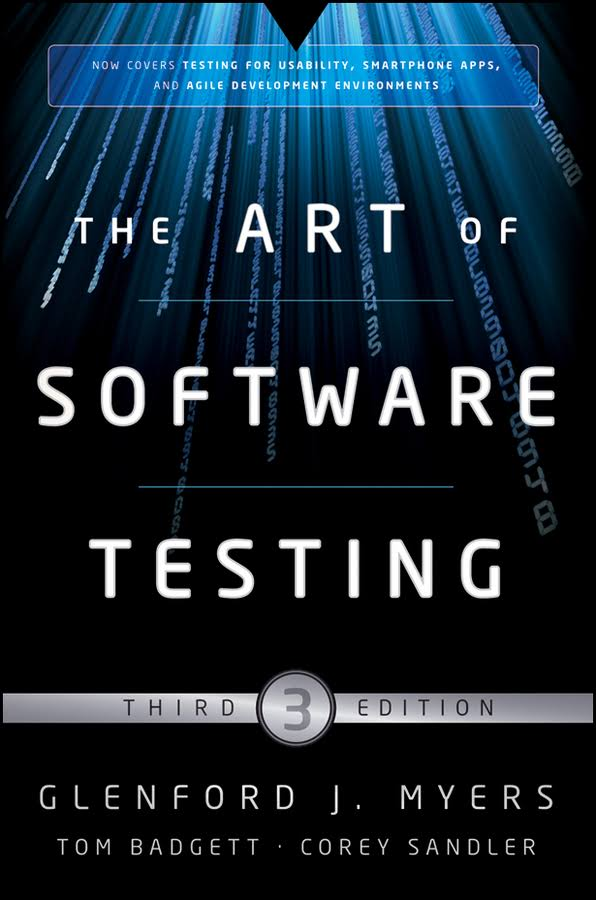
\includegraphics[height=28mm]{SoftwareTesting.jpeg}\hfill
                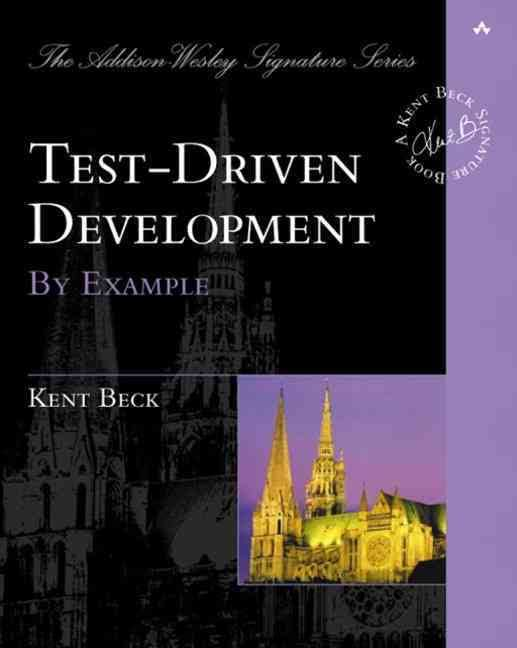
\includegraphics[height=28mm]{TDD.jpeg}
            \end{itemize}
        \end{column}
        \begin{column}{0.55\textwidth}
            \begin{itemize}
                \item \PP{Testing types and techniques}
                \begin{itemize}
                    \item \textcolor{bg!80!normal text.fg}{Manual testing}
                    \item \PS{Automated testing}
                    \item Continuous testing
                    \item Functional testing
                    \item Mutation testing
                    \item Fuzzy testing
                    \item \ldots
                \end{itemize}
                \vspace{2mm}
                \item \small \PB{Plenty of videos/resources on the web}
            \end{itemize}
            \begin{itemize}
                \scriptsize\setlength{\itemsep}{0mm}
                \item[]
                \URL{https://www.youtube.com/watch?v=u5senBJUkPc}{~CppCon2015 -- All your tests are terrible\ldots}
                \item[]
                \URL{https://www.youtube.com/watch?v=FjwayiHNI1w}{~CppCon2020 -- The science of unit tests}
                \item[]
                \URL{https://www.youtube.com/watch?v=_OHE33s7EKw}{~CppCon2020 -- Back to Basics: Unit Tests}
                \item[]
                \URL{https://www.youtube.com/watch?v=EZ05e7EMOLM}{~TDD, Where Did It All Go Wrong}
                \item[] \ldots
            \end{itemize}
        \end{column}
    \end{columns}
    \FrameRemark{The videos linked here above (as well as the references therein) were mainly used to prepare this talk.}
\end{frame}
%~~~~~~~~~~~~~~~~~~~~~~~~~~~~~~~~~~~~~~~~~~~~%
%Tikz group of commands to make a pyramid layer
\newcommand{\pyramidLayer}[6][]{%
    \pgfmathsetmacro{\Thickness}{#3}
    \pgfmathsetmacro{\Long}{#4}
    \pgfmathsetmacro{\Short}{#4-0.5*#3}
    \path coordinate (middleUpperRight) at ($(#2)+(0,\Thickness)+(30:0.5*\Short)$)
    coordinate (middleLowerRight) at ($(#2)+(30:0.5*\Long)$)
    coordinate (upperRight) at ($(#2)+(0,\Thickness)+(30:\Short)$)
    coordinate (lowerRight) at ($(#2)+(30:\Long)$);
    \draw[fill=#5!50] ($(#2)+(0,\Thickness)+(30:\Short)$)  -- ++(210:\Short) -- ++(270:\Thickness) -- ++(30:\Long) -- cycle;
    \draw[fill=#5!20] ($(#2)+(0,\Thickness)+(150:\Short)$)  -- ++(330:\Short) -- ++(270:\Thickness) -- ++(150:\Long) -- cycle;
    \draw[fill=#5]    ($(#2)+(0,\Thickness)$) -- ++(30:\Short) -- ++(150:\Short) -- ++(210:\Short) -- cycle;
    \node[font=\small] at ($(middleUpperRight)!0.5!(middleLowerRight)$) {\rotatebox{30}{#6}};
    \node[text=#5, anchor=west] at ($(upperRight)!0.5!(lowerRight)+(0.5,0)$) {#1};
}
\begin{frame}{The tests pyramid}
    \begin{center}
        \resizebox{!}{0.8\textheight}{
            \begin{tikzpicture}
                \path coordinate (A) at (0,0)
                      coordinate (B) at (0,2)
                      coordinate (C) at (0,4)
                      coordinate (D) at (0,6)
                      coordinate (O) at ($(A)+(150:5)-(0.5,0)$);
                \draw (O) -- ++(30:2); %Just draw axis behind pyramid
                %Draw Pyramid
                \pyramidLayer{A}{1.5}{5}{red}{Unit};
                \pyramidLayer{B}{1.5}{4}{orange!80!yellow}{Integration};
                \pyramidLayer{C}{1.5}{3}{PS}{System};
                \pyramidLayer{D}{1.5}{2}{PP}{Acceptance};
                \draw[to] (O) -- ++(0,6) node[right, anchor=north west] {Execution time};
                \draw[to] (O) -- ++(330:6) node[right] {Number of tests};

            \end{tikzpicture}
        }
    \end{center}
\end{frame}
%~~~~~~~~~~~~~~~~~~~~~~~~~~~~~~~~~~~~~~~~~~~~%
\begin{frame}{Unit tests are not enough!}
    \begin{varblock}{}[0.9\textwidth]{Integration tests}
        \PB{Once you are sure that all components work correctly alone, be sure they work as expected together!}
    \end{varblock}
    \vspace{3mm}
    \begin{overlayarea}{\textwidth}{0.8\textheight}
        \begin{center}
            \begin{onlyenv}<1>
                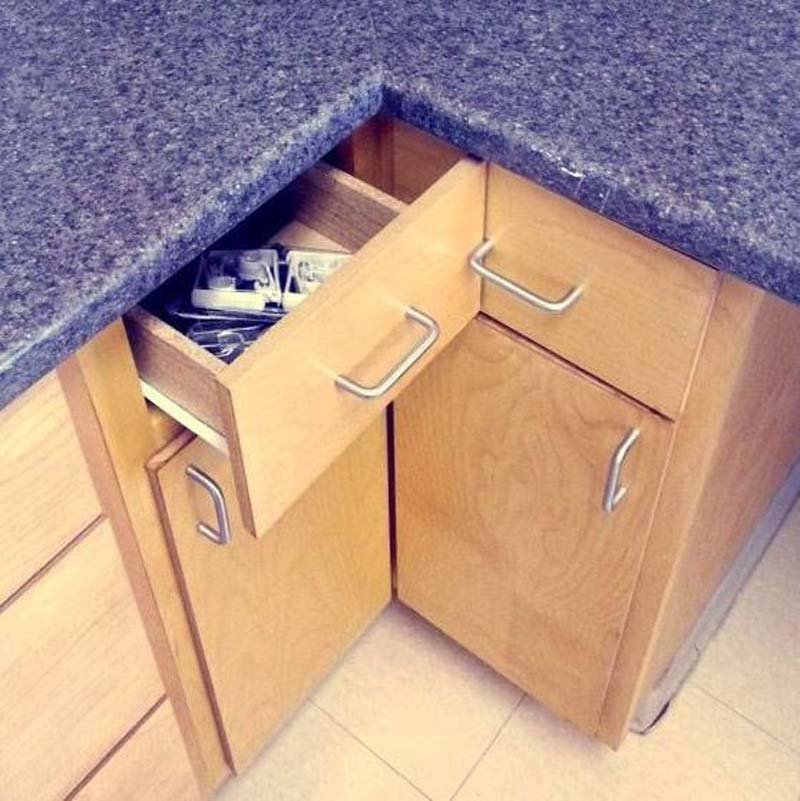
\includegraphics[height=4cm]{UnitTestVSIntegrationTestA}$\quad$
                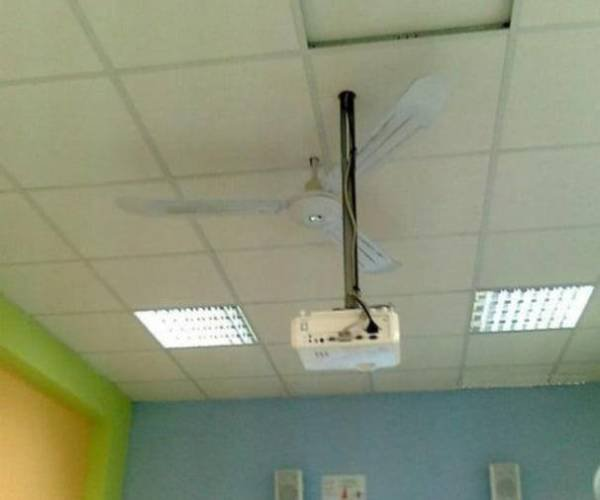
\includegraphics[height=4cm]{UnitTestVSIntegrationTestB}\\
            \end{onlyenv}
            \begin{onlyenv}<2>
                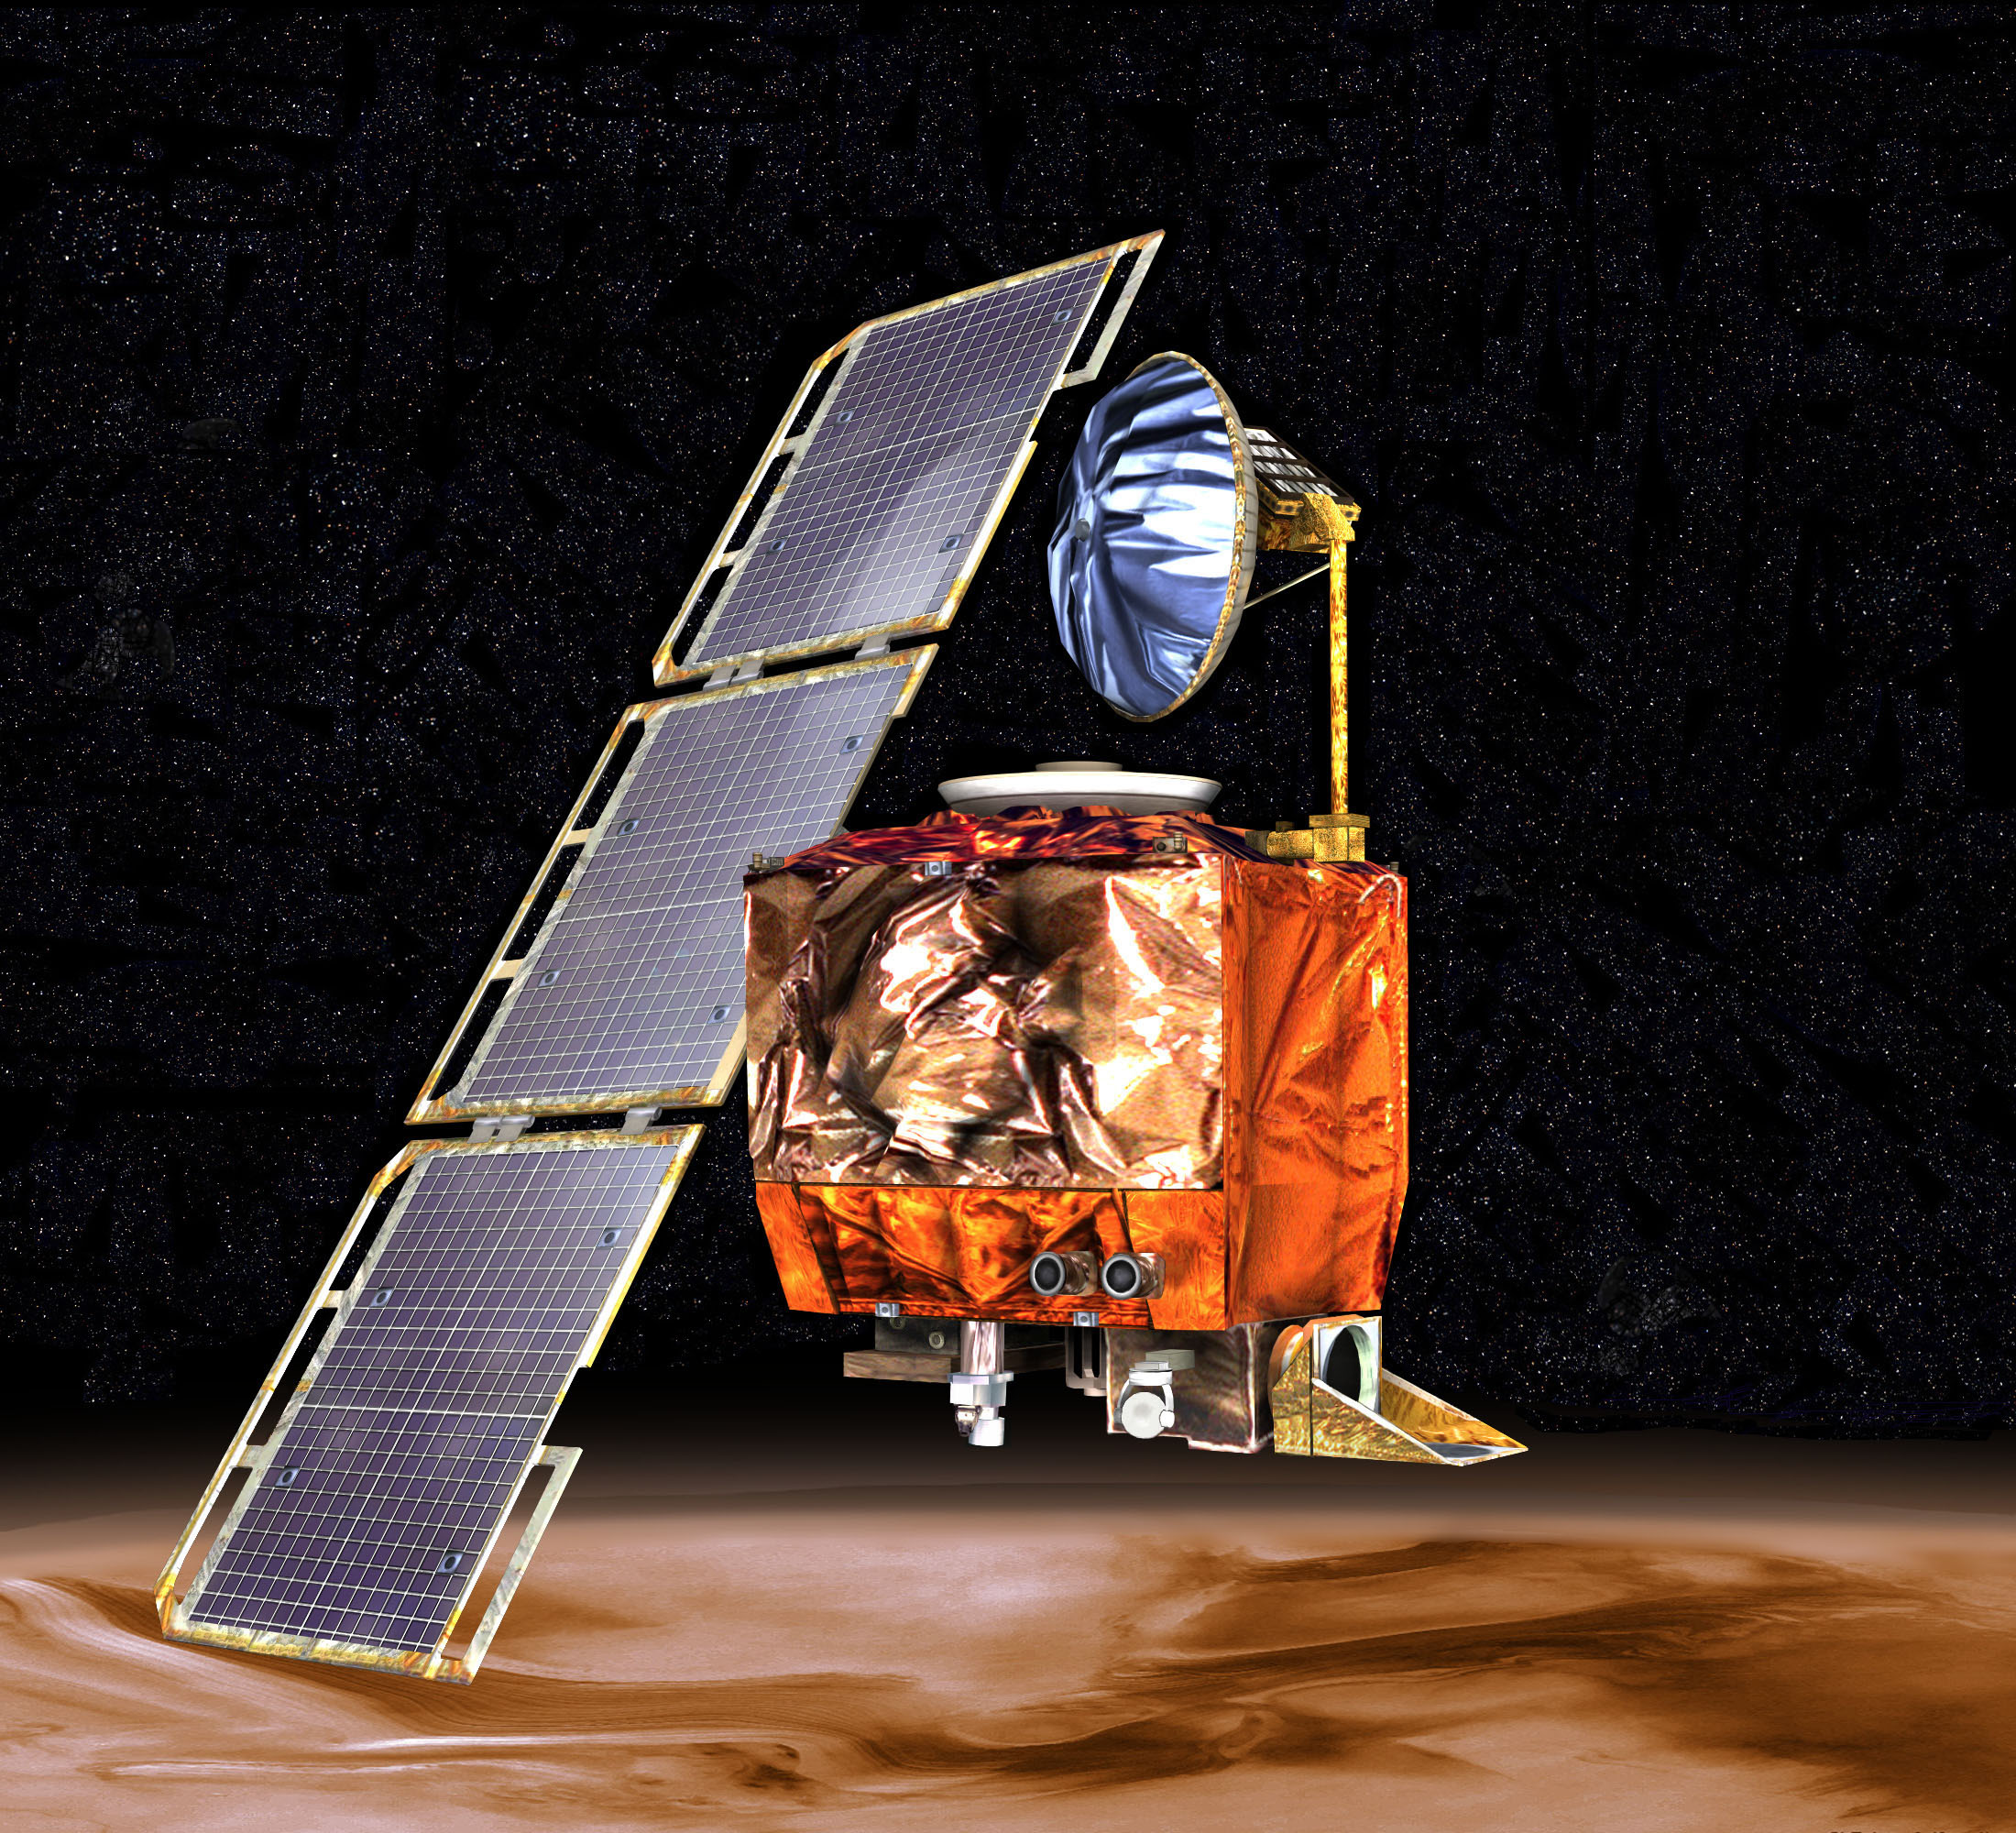
\includegraphics[height=35mm]{MarsClimateOrbiter}\\
                {
                    \scriptsize
                    \URL[PB]{http://www.vitalstatistics.info/uploads/mars\%20climate\%20orbiter.jpg}{Mars Climate Orbiter}
                    lost in 1999 -- By NASA/JPL/Corby Waste -- \myCopyright\ Public Domain
                }
            \end{onlyenv}
        \end{center}
    \end{overlayarea}
    \FrameRemark{I already mentioned this in the \textsl{Clean code} talk.}
\end{frame}
%===================================================================================================%
\end{comment}


%===================================================================================================%
\section{Tests goals -- properties -- good principles}
%~~~~~~~~~~~~~~~~~~~~~~~~~~~~~~~~~~~~~~~~~~~~%
\begin{frame}{General idea and overview}
    \begin{overlayarea}{\textwidth}{0.7\textheight}
        \begin{center}
            \large
            \only<1-2>{There is slightly different advice around, pick your favourite:}
            \only<3->{There is one not-negotiable \textbf{requirement of tests}, though:}
        \end{center}
        \begin{varblock}{example}[0.8\textwidth]{Write F.I.R.S.T tests first}<only@1>
            \begin{description}[Self-validating:]
                \item[\PQ{F}ast:] To be run frequently
                \item[\PQ{I}ndependent:] To make failures meaningful
                \item[\PQ{R}epeatable:] To be run everywhere with same outcome
                \item[\PQ{S}elf-validating:] To be automatised
                \item[\PQ{T}imely:] To make production code testable
            \end{description}
        \end{varblock}
        \begin{varblock}{example}[\textwidth]{Google's perspective}<only@2>
            \begin{description}[Self-validating:]
                \item[Readable:] Tests are correct by inspection
                \item[Correct:] Do not rely on known bugs and test real scenarios
                \item[Complete:] Test most edge cases
                \item[Documenting:] Demonstration of how the API works
                \item[Resilient:] Repeatable, independent, hard to break, hermetic, etc.
            \end{description}
        \end{varblock}
        \begin{tikzpicture}[overlay, remember picture]
            \node[starburst, starburst points=21, starburst point height=15mm,
                  minimum width=10cm, minimum height=6cm, Shape={red}{yellow!50}{red},
                  line width=1.5pt, font=\Huge\bfseries, visible on=<4>]
                at ($(current page.center)-(0,1)$) {Existence};
        \end{tikzpicture}
    \end{overlayarea}
\end{frame}
%~~~~~~~~~~~~~~~~~~~~~~~~~~~~~~~~~~~~~~~~~~~~%
\begin{frame}[fragile]{A small interlude: Unit test frameworks}{Essential for self-validation and automation!}
    \vspace{-2mm}
    \begin{overlayarea}{\textwidth}{0.7\textheight}
        \begin{enumerate}[<+->]
            \item Boost Test Library\hfill
                  \parbox{0.3\textwidth}{\footnotesize\URL[PB]{https://www.boost.org/doc/libs/1_82_0/libs/test/doc/html/index.html}{Documentation}}
                  \begin{varblock}{example}[0.9\textwidth]{}<only@1>
                      \begin{lstlisting}[style=MyCpp]
                          #define BOOST_TEST_MODULE My Test
                          #include |+<boost/test/included/unit_test.hpp>+|

                          BOOST_AUTO_TEST_CASE(first_test)
                          {
                              int i = 1;
                              BOOST_TEST(i);
                              BOOST_TEST(i == 2);
                          }
                      \end{lstlisting}
                      \begin{lstlisting}[style=MyBash]
                          |+Running 1 test case...
                          test_file.cpp(8): error: in "first_test": check i == 2 has failed [1 != 2]

                          *** 1 failure is detected in the test module "My Test"+|
                      \end{lstlisting}
                  \end{varblock}
            \item GoogleTest\hfill
                  \parbox{0.3\textwidth}{\footnotesize\URL[PB]{https://google.github.io/googletest/}{User's guide}}
                  \begin{varblock}{example}[0.9\textwidth]{}<only@2>
                      \begin{lstlisting}[style=MyCpp]
                          #include |+<gtest/gtest.h>+|
                          #include |+"src/factorial.h"+|

                          TEST(FactorialTest, HandlesZeroInput) {
                              EXPECT_EQ(factorial(0), 1);
                          }

                          TEST(FactorialTest, HandlesPositiveInput) {
                              EXPECT_EQ(factorial(1), 1);
                          }

                          int main(int argc, char **argv) {
                              ::testing::InitGoogleTest(&argc, argv);
                              return RUN_ALL_TESTS();
                          }
                      \end{lstlisting}
                  \end{varblock}
            \item Vir's Unit Test Framework\hfill
                  \parbox{0.3\textwidth}{\footnotesize\URL[PB]{https://github.com/mattkretz/virtest}{GitHub repository}}
                  \begin{varblock}{example}[0.9\textwidth]{}<only@3>
                      \begin{lstlisting}[style=MyCpp]
                          #include |+<vir/test.h>+|

                          TEST(test_name) {
                              int test = 3;
                              COMPARE(test, 2) << "more " << "details";
                              //COMPARE(test, 2).on_failure("more ", "details");
                          }
                      \end{lstlisting}
                      \begin{lstlisting}[style=MyBash]
                          @|\tikzmark{corner}|@|+FAIL:  at tests/testfile.cpp:5 (0x40451f):
                          FAIL:  test (3) == 2 (2) -> false more details
                          FAIL:  test_name

                          Testing done. 0 tests passed. 1 tests failed.+|
                      \end{lstlisting}
                  \end{varblock}
            \item {\small ...and so many mores!}\hfill
                  \parbox{0.3\textwidth}{\footnotesize\URL[PB]{https://en.wikipedia.org/wiki/List_of_unit_testing_frameworks\#C++}{List on Wikipedia}}
        \end{enumerate}
        \vspace{1mm}
        \begin{varblock*}{alert}[0.8\textwidth]{Not all have the same weight and functionality}<only@4>
            Pick your favourite depending on your needs and project:
            \vspace{2mm}
            \begin{enumerate}
                \small
                \item Natural choice if you already depend on Boost
                \item More complex but also more powerful
                \item Very simple and lightweight
            \end{enumerate}
        \end{varblock*}
        \begin{tikzpicture}[remember picture, overlay]
            \draw[thick, visible on=<3>] ($(corner)-(0.335\textwidth,0.13)$) -- ++(-0.12,0) -- ++(0,-0.68) -- ++(0.12,0);
        \end{tikzpicture}
    \end{overlayarea}
\end{frame}
%~~~~~~~~~~~~~~~~~~~~~~~~~~~~~~~~~~~~~~~~~~~~%
\begin{frame}[fragile]{Having tests is not enough, you must trust them!}{Few words about tests correctness}
    \begin{overlayarea}{\textwidth}{0.7\textheight}
        \begin{itemize}
            \item Never rely on known bugs
            \item<only@4-> Never mock the code that you are testing
        \end{itemize}
        \begin{varblock}{alert}[0.6\textwidth]{Having tests passing is simple...}<only@1-2>
            \begin{uncoverenv}<2->
                \begin{lstlisting}[style=MyCpp]
                    int cube(int x) {
                        //TODO: To be implemented
                        return 0;
                    }

                    TEST(cube_test) {
                        VERIFY(0 == cube(2));
                        VERIFY(0 == cube(3));
                        VERIFY(0 == cube(42));
                    }
                \end{lstlisting}
            \end{uncoverenv}
        \end{varblock}
        \begin{varblock}{example}[0.6\textwidth]{...better to have them failing!}<only@3>
            \begin{lstlisting}[style=MyCpp]
                int cube(int x) {
                    //TODO: To be implemented
                    return 0;
                }

                TEST(cube_test) {
                    VERIFY(8 == cube(2));
                    VERIFY(27 == cube(3));
                    VERIFY(74088 == cube(42));
                }
            \end{lstlisting}
        \end{varblock}
        \begin{varblock}{example}[0.8\textwidth]{This is probably useless}<only@4>
            \begin{lstlisting}[style=MyCpp]
                class MockCoffeeMachine : public CoffeeMachine {
                    //For simplicity we assume always in temperature
                    double warmUp() override {
                        return constants::brewingT;
                    }
                }

                BOOST_AUTO_TEST_CASE(warmUp_test) {
                    MockCoffeeMachine machine{};
                    BOOST_REQUIRE_CLOSE(machine.warmUp(),
                                        constants::brewingT, 0.1);
                }
            \end{lstlisting}
        \end{varblock}
        \vspace{3mm}
        \begin{varblock}{}[0.85\textwidth]{Think of a clear reaction procedure in your team}<only@5->
            What should happen in your project when a test fails?\\
            ...and when a bug that was not caught by tests is found?\\
            $\downarrow$\\
            \PB{Never miss any chance to improve your tests!}
        \end{varblock}
    \end{overlayarea}
\end{frame}
%~~~~~~~~~~~~~~~~~~~~~~~~~~~~~~~~~~~~~~~~~~~~%
\begin{frame}{Tests readability}
    \begin{center}
        \begin{tikzpicture}[every node/.style={inner sep=0mm, text=BGLIGHT}]
            \node (fig) {
\includegraphics[width=0.75\textwidth]{Balance}};
            \begin{DrawOnNode}{fig}
                \node[anchor=east] at (0.41,0.78) {
                    \begin{tabular}{c}
                        Avoid boilerplate\\
                        \footnotesize E.g. use functions for setup\\
                    \end{tabular}
                };
                \node[anchor=west] at (0.51,0.78) {
                    \begin{tabular}{c}
                        Give enough context\\
                        \footnotesize E.g. Not a single function for setup\\
                    \end{tabular}
                };
            \end{DrawOnNode}
        \end{tikzpicture}
    \end{center}
    \begin{varblock}{}[0.85\textwidth]{}
        \Large Remember: \PB{Tests are correct by inspection!}
    \end{varblock}
\end{frame}
%~~~~~~~~~~~~~~~~~~~~~~~~~~~~~~~~~~~~~~~~~~~~%
\begin{frame}[fragile]{Tests completeness: What should I test and how?}
    \begin{onlyenv}<1>
        \begin{itemize}
            \item Values  \\ \centerline{
\includegraphics[scale=0.1]{TestingValue}}
            \item Actions \\ \centerline{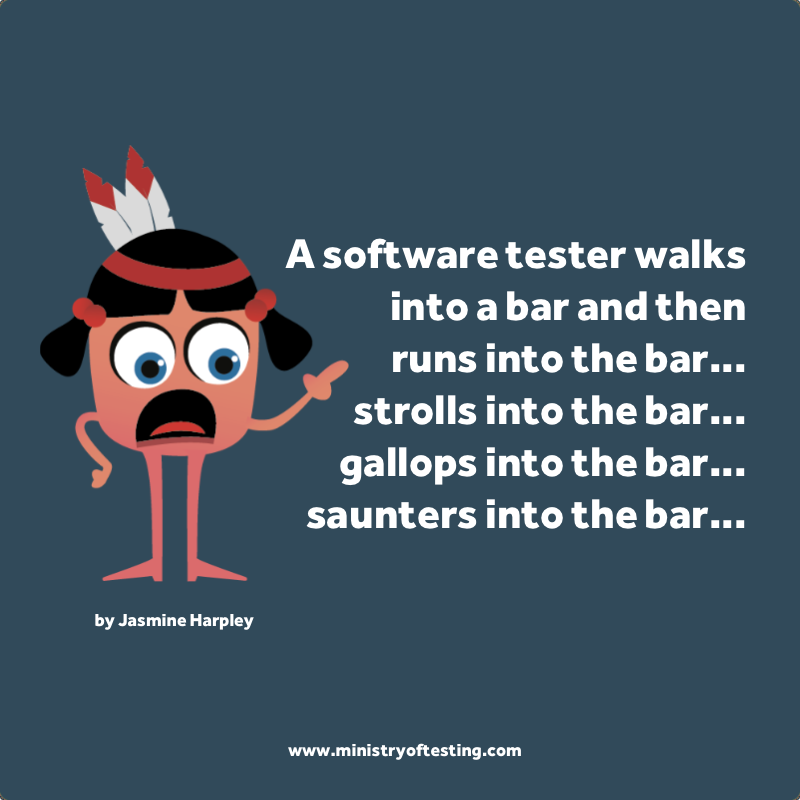
\includegraphics[scale=0.12, clip, trim=0 4cm 0 4cm]{TestingAction}}
        \end{itemize}
        \vspace{3mm}
        \hfill\ldots{}and anything that makes sense!
    \end{onlyenv}
    \begin{varblock}{example}[0.98\textwidth]{A very nice example from Titus Winter}<only@2->
        \begin{overlayarea}{\textwidth}{0.55\textheight}
            \begin{uncoverenv}<3->
                \begin{lstlisting}[style=MyCpp]
                    int Factorial(int n) {
                        if (n == 1) return 1;
                        if (n == 5) return 120;
                        return -1; // TODO(goofus): figure this out.
                    }
                \end{lstlisting}
            \end{uncoverenv}
            \begin{onlyenv}<2-3>
                \begin{lstlisting}[style=MyCpp]
                    TEST(FactorialTest, BasicTests) {
                        EXPECT_EQ(1, Factorial(1));
                        EXPECT_EQ(120, Factorial(5));
                    }
                \end{lstlisting}
            \end{onlyenv}
            \begin{onlyenv}<4>
                \begin{lstlisting}[style=MyCpp]
                    TEST(FactorialTest, BasicTests) {
                        EXPECT_EQ(1, Factorial(1));
                        EXPECT_EQ(120, Factorial(5));
                        EXPECT_EQ(1, Factorial(0));
                        EXPECT_EQ(479001600, Factorial(12));
                        EXPECT_EQ(std::numeric_limits::max<int>() , Factorial(13));
                        EXPECT_EQ(1, Factorial(0));
                        EXPECT_EQ(std::numeric_limits::max<int>() , Factorial(-10));
                    }
                \end{lstlisting}
            \end{onlyenv}
        \end{overlayarea}
    \end{varblock}
    \begin{uncoverenv}<4>
        \begin{center}
            This will pretty much naturally emerge when doing TDD
        \end{center}
    \end{uncoverenv}
\end{frame}
%~~~~~~~~~~~~~~~~~~~~~~~~~~~~~~~~~~~~~~~~~~~~%
\begin{frame}{The hidden value of tests}{Few words about tests as API usage examples}
    \begin{center}
        \small
        Of course, a meme, do not take it seriously, but...\\
        \bigskip
        
\includegraphics[width=0.7\textwidth]{Documentation_meme}\\
        \bigskip
        ...good tests should show how to use your code!
    \end{center}
    \FrameRemark{In this sense, it should be avoided to use implementation details in tests (cf. white box testing downsides).}
\end{frame}
%~~~~~~~~~~~~~~~~~~~~~~~~~~~~~~~~~~~~~~~~~~~~%
\begin{frame}[fragile]{Tests resilience: Google advice}
    \begin{onlyenv}<1>
        \begin{itemize}
            \setlength{\itemsep}{2mm}
            \item No flaky tests $\to$ Tests should always give the same outcome
            \item No brittle tests $\to$ One failure should not trigger many failures
            \item Tests reference values should not come from the system under test!
            \item Changing tests order should never change the outcome
            \item Tests should be as hermetic as possible $\to$ No I/O, no network, etc.
            \item No deep dependence $\to$ Avoid any implicit assumption
        \end{itemize}
        \vspace{3mm}
        \begin{varblock}{example}[0.5\textwidth]{}
            \large Let's see some examples!
        \end{varblock}
    \end{onlyenv}
    \begin{onlyenv}<2-3>
        \begin{varblock}{example}[\textwidth]{A sneaky flaky test}
            \begin{lstlisting}[style=MyCpp]
                TEST(UpdaterTest, RunsFast) {
                    Updater updater;
                    updater.UpdateAsync();
                    SleepFor(Seconds(.5)); // Half a second should be *plenty*.
                    EXPECT_TRUE(updater.Updated());
                }
            \end{lstlisting}
        \end{varblock}
        \begin{varblock}{example}[\textwidth]{An infamous brittle pattern}<uncover@3>
            \begin{lstlisting}[style=MyCpp]
                TEST(Logger, LogWasCalled) {
                    StartLogCapture();
                    EXPECT_TRUE(Frobber::Start());
                    EXPECT_THAT(
                      Logs(), Contains("file.cc:421: Opened file frobber.config" )
                    );@|\tikzmark{logger}|@
                }
            \end{lstlisting}
        \end{varblock}
        \begin{tikzpicture}[remember picture, overlay]
            \draw[red, thick, double, visible on=<3>]
                ($(logger)-(2.6,0)$) -- ++(1.15,0)
                +(0.18,0) -- ++(0.65,0)
                +(2.4,0) -- ++(4.8,0);
        \end{tikzpicture}
    \end{onlyenv}
    \begin{onlyenv}<4-5>
        \begin{varblock}{example}[\textwidth]{Where are the reference values coming from?}
            \begin{lstlisting}[style=MyCpp]
                BOOST_AUTO_TEST_CASE(Dirac_M)
                {
                    const hmc_float refs[4] =
                        { 2610.3804893063798, 4356.332327032359,
                          2614.2685771909237, 4364.1408252701831 };
                    test_fermionmatrix<physics::fermionmatrix::Dslash>(refs);
                }
            \end{lstlisting}
        \end{varblock}
        \begin{varblock}{example}[\textwidth]{A non-hermetic test: What if run twice in parallel?}<uncover@5>
            \begin{lstlisting}[style=MyCpp]
                TEST(Server, StorageTest) {
                    StorageServer* server = GetStorageServerHandle();
                    auto my_val = rand();
                    server->Store("testkey", my_val);
                    EXPECT_EQ(my_val, server->Load("testkey"));
                }
            \end{lstlisting}
        \end{varblock}
    \end{onlyenv}
    \begin{onlyenv}<6>
        \vspace{-3mm}
        \begin{varblock}{example}[\textwidth]{Deep dependence example}<only@6>
            \begin{lstlisting}[style=MyCpp]
                class File {
                  public:
                    // ...
                    virtual bool StatWithOptions(Stat_t* stat, StatOptions opts) {
                        return this->Stat(stat); // In base class ignore options
                    }
                };
                TEST(Filesystem, FSUsage) {
                    // ... and call to StatWithOptions
                    EXPECT_CALL(file, Stat(_)).Times(1);
                }  // This relies on a call to base StatWithOptions!!
            \end{lstlisting}
        \end{varblock}
        \begin{varblock}{quote}[\textwidth]{The law of implicit interfaces (AKA Hyrum's law)}[Hyrum Wright]<only@6>
            Given enough users of your public interface, soon or later someone will start implicitly relying on your implementation details (speed, memory consumption, etc.).\\[-1.5ex]~
        \end{varblock}
    \end{onlyenv}
    \FrameRemark{This list and all GoogleTest example are taken from Titus Winters' and Hyrum Wright's talk at CppCon2015.}
\end{frame}
%===================================================================================================%


%===================================================================================================%
\section[White and black box testing]{The weaknesses of white and black box testing}
%~~~~~~~~~~~~~~~~~~~~~~~~~~~~~~~~~~~~~~~~~~~~%
% - White box -> we tighten testing and production code e.g. with friends
%   (sometimes neede -> start to test legacy code)
% - Black box -> at some point testing a method we rely on correctness of other methods
%    => The fragile test problem (also more in general, one failure -> many failures)
%===================================================================================================%

% Mutation testing
% What is right? -> Numerical precision to be wisely chosen
%   -> e.g. FMA could make your test fail if you require too high precision
% Reproducibility
% 1. Isolation -> Mocking
% 2. Subtraction -> Measure unwanted environment effect, correct tests to compensate
% 3. Detect and respond -> Implement functionality to detect if test can be run, if not do something
% 4. Statistics -> E.g. no PRNG, but if needed, measure failure frequency and enforce it in code
%   -> a failure of a test must be a failure, i.e. something to react on!
% Accuracy -> Window with four cases Code correct/wrong VS tests pass/fail

%===================================================================================================%
\section[BDD in its original idea]{Behaviour driven development in its original idea}
%~~~~~~~~~~~~~~~~~~~~~~~~~~~~~~~~~~~~~~~~~~~~%
%===================================================================================================%


%===================================================================================================%
\section{Test driven development as discipline}
%~~~~~~~~~~~~~~~~~~~~~~~~~~~~~~~~~~~~~~~~~~~~%
%===================================================================================================%


%===================================================================================================%
\section{What to do, now?}
%~~~~~~~~~~~~~~~~~~~~~~~~~~~~~~~~~~~~~~~~~~~~%
%===================================================================================================%

\end{document}
